\documentclass{thesis}


\usepackage{url}
% TX Fonts を使う
\usepackage{listings,jvlisting}
\usepackage{txfonts}
\usepackage{ascmac}
\usepackage{listings,jvlisting}
\usepackage{lineno}
\usepackage{indentfirst}

\renewcommand{\lstlistingname}{プログラム}
\begin{document}

\lstset{
  basicstyle={\ttfamily},
  identifierstyle={\small},
  commentstyle={\smallitshape},
  keywordstyle={\small\bfseries},
  ndkeywordstyle={\small},
  stringstyle={\small\ttfamily},
  frame={tb},
  breaklines=true,
  columns=[l]{fullflexible},
  numbers=left,
  xrightmargin=0zw,
  xleftmargin=3zw,
  numberstyle={\scriptsize},
  stepnumber=1,
  numbersep=1zw,
  lineskip=-0.5ex
}

% 目次
\tableofcontents

\chapter{序論}

%近年では、インターネット技術や各種センサ・テクノロジーの進化等を背景に、パソコンやスマートフォンなどの従来のインターネット接続端末加え、駆動装置、建物、自動車、家電製品、電子機器など、世界中の様々なモノがインターネットにつながるようになっている。
%総務省による世界のIoTデバイス数の推移および予測によると、世界のIoTデバイス数は2016年では173.2億台、
%2018年では208.7億台、2020年では253.0億台となっている\cite{令和3年版情報通信白書}。またIoT機器の増加、インターネットの発展に伴い、サイバー攻撃も増加し,情報通信研究機構(NICT)が運用するサイバー攻撃観測網(NICTER)が2020年(令和2年)に観測したサイバー攻撃関連通信についても、約4割がIoT機器を狙ったものであるという結果が示されている\cite{サイバー攻撃の最近の動向等について}。そのため、大きな問題となっているのがIo Tのセキュリティ対策である。家電、スマートグリッドなどのような処理能力の高いIoT機器だけでなく、湿度センサやICタグなど小型で低スペックのIoT機器にも適用できるようなセキュリティ対策が不可欠で、従来の情報技術とは異なるアプローチが必要になる。

%その中で2018年に、IoTセキュリティの一技術としてSAS-L(Simple And Secure password authentication protocol,Light processing version)が新たに考案された。SAS-Lとは、高知工科大学の清水明宏教授らが開発したワンタイムパスワード認証方式の1つである。特徴は、従来最高速であるワンタイムパスワード認証方式SAS-2に比較して、更に高速で、特に、認証側あるいは被認証側において、処理負荷の大きい一方向性変換関数の適用を必要としない、すなわち、処理負荷がほぼゼロに近い方式である\cite{SAS-Lワンタイムパスワード認証方式について}。そのため、センサやICタグのように小型かつ低スペックのIoT機器に搭載可能である。SAS-LにはバージョンとしてSAS-L(1),(2),(3),(4)といったものがある。SAS-L(1),(2),(4)に関しては安全性と計算機実験について評価が行われている。しかし、SAS-L(3)に関しては安全性と計算機実験の評価が未検証である。

%そのため、本研究ではSAS-L(3)の安全性と実用性の検証を行うことを目的とする。比較対象として、類似しているSAS-L(4)も同じ環境に実装を行い、SAS-L(3)の有効性を評価する。評価項目としては、CPU計算時間とする。第1章では、研究の背景および目的について述べる。 第2章では、実装したプログラム内で用いた要素技術の原理について述べる。第3章ではSAS-L(3)およびSAS-L(4)の原理について述べる。第4章では、実装したシステムについて述べる。第5章では、実装したシステムを用いた評価実験の方法および結果を示した後、実験結果に基づいた考察を述べる。第6章では、本研究のまとめおよび今後の課題を述べる。


近年、インターネット技術の発展により、従来のPCやス
マホ端末に加え、自動車、家電製品、建物など、世界中
の様々なものがインターネットに接続されている。イン
ターネットに接続されたIoT 機器の増加にともない、サ
イバー攻撃への対応が大きな問題になっている。
実際、情報通信研究機構(NICT)が運用するサイバー攻
撃観測網(NICTER)が2020年(令和2 年)に観測したサ
イバー攻撃の統計結果\cite{サイバー攻撃の最近の動向等について}によると、約4 割がIoT 機器を狙
ったものであるという結果が示されている。
IoT 機器はPCなどに比べると処理能力が低いため、安全
性を確保しつつ処理コストをおさえたセキュリティ対策
が必要である。

本研究では、IoTのための認証手法として、SAS-L(Simple 
And Secure password
authentication protocol,Light processing version)\cite{SAS-Lワンタイムパスワード認証方式について}
について検討する。SAS-L とは、高知工科大学の清水明
宏教授が開発したワンタイムパスワード認証方式である。
特徴は、従来のワンタイムパスワード認証方式SAS-2 に
比較して、更に処理コストが低いであることである。特
に、認証側あるいは被認証側において、処理負荷の大き
い一方向性関数の適用を必要としない。センサ
やIC タグのような小型かつ低スペックのIoT 機器に搭
載可能である。

SAS-L には、SAS-L(1)~(4) という4種類のバージョン
が提案されている。このうち被認証側で一方向性関数を
必要としないのはSAS-L(3)とSAS-L(4)である。SAS-L(4)
については実装実験が行われているが、SAS-L(3)につい
ては実装による評価はされていない。そこで、本研究で
はSAS-L(3)の実装および安全性に関する検討を行い、
類似しているSAS-L(4)と比較しながらSAS-L(3)の有効性について検証する。

第1 章では、研究の背景および目的について述べる。
第2 章では、SASで用いられる暗号技術について述べる。
第3 章ではSAS-L(3) およびSAS-L(4) のプロトコルにつ
いて述べる。
第4 章では、評価実験の方法および結果を示す。
第5 章では、本研究のまとめおよび今後の課題を述べる。
%-------------------------------------------------------------------------------------------
%-------------------------------------------------------------------------------------------
%-------------------------------------------------------------------------------------------

\chapter{ワンタイムパスワード認証と暗号技術}

\section{ワンタイムパスワード認証方式}
ワンタイムパスワード認証\cite{認証技術}とは、ワンタイム(1度だけ)、あるいは短期間だけ使用できるパスワードを利用した認証である。
認証の度に認証情報が変化するため、不正ログイン、第3者によるなりすましの防止などのセキュリティ強化が期待できる。
ワンタイムパスワードを生成するには、大きく2つ方法がある。カウンタベースのトークンでは、ベースシークレットを同期カウンタと組み合わせてワンタイムパスワードを生成する。クロックベースのトークンでは、同期クロックを使ってワンタイムパスワードを生成する。これらの手法はすべて、ワンタイムパスワードトークン内に格納されているランダムなベースシークレットを利用する。このベースシークレットを何らかの任意の値(カウンタ、クロック、またはその両方と組み合わせることで、新しいパスワードを生成する。


%ランポート数式で!!!!!  論文として発表の参考文献
\subsection{S/Key認証}
S/Key\cite{s/key}とは、Unixシステム用のログオン技術として1990年代はじめにBellcore社が開発したワンタイムパスワードシステムである。
技術的なコンセプトを最初に提案したのはLeslie Lamportで、これは1981年に論文\cite{Lamport}として発表された。
Lamportの方式では、ハッシュ関数を使ってサーバにパスワードを保存するため、パスワードをそのまま保存しない。また、認証の度に異なる情報が通信される特徴を持つ。Lamportの方式の手順を以下に示す。

\textgt{初期化}
\begin{enumerate}[・]
\item ユーザは乱数$x$を選択
\item ユーザはハッシュ関数Fを使って次の値を計算してサーバに安全な通信路で送信($y_i$は$i$回目の認証情報)

$y_{1} = F^{1000},y_{2} = F^{999}(x),…,y_{1000} = F^1(x)$
\end{enumerate}
\textgt{認証手順}
\begin{enumerate}[・]
\item ユーザは、$x_i = F^{1000-i}(x)$をサーバに送信
\item サーバで$F(x_i)$を計算し、$y_i$と比較
\end{enumerate}
認証手順を繰り返すと、最終的には$x_{1000} = F^1(x)$をユーザからサーバに送信するところで、再利用可能なパスワードが尽きてしまう。そのため、この段階でもう一度初期化処理を行う。



%Lamportのアプローチでは秘密鍵のデータベースを使用しないので、攻撃者にベースシークレットのデータベースが盗まれてシステムが危険にさらされるという心配がない。Lamportの手法では、人間が記憶しているパスワードから一連の一方向ハッシュ値を計算する。伝統的なUnixパスワードと同様に、このシステムは、パスワードのハッシュを計算するのは容易でも、ハッシュからパスワードを逆算するのは事実上不可能であるという性質を利用している。Lamportの方法では、ハッシュから2番目のハッシュを計算し、2番目のハッシュから3番目のハッシュ計算するという具合に一連のハッシュを生成し、そのうち最後のハッシュをサーバに格納する。

%図がいるかも

%ユーザはログオンに際して、最後から2番目のハッシュをワンタイムパスワードとして入力する。サーバは入力されたワンタイムパスワードをハッシュし、その結果を格納されているハッシュと比較する。両者が一致した場合、サーバはユーザのパスワードエントリ内にあるハッシュを、ユーザがいま入力したパスワードに置き換える。次にログオンするとき、ユーザは2番目のハッシュを入力し、サーバは同じプロセスを繰り返す\cite{認証技術}。

\section{ハッシュ関数}
ハッシュ関数\cite{ハッシュ関数}とは、任意長のメッセージを入力すると、メッセージを代表する固定長の値を出力する関数である。ハッシュ関数の出力値をハッシュ値と呼ぶ。入力サイズが小さくても大きくても、出力サイズは一定になる。また、同じハッシュ関数に同じメッセージが入力されたとき、同じハッシュ値が出力されなければならない。さらに、入力値が大きくても高速でハッシュ値が計算できることが求められる。そのため、ハッシュ関数はリアルタイムな処理に使用できる。

\subsection{ハッシュ関数の安全性}
ハッシュ関数の標準的な安全性として、次の3つが挙げられる。
\begin{enumerate}[・]
\item \textgt{ 一方向性(原像計算困難性)}

一方向性とは、ハッシュ値が与えられたとき、元のメッセージを求めることが困難であることである。原像計算困難性とも呼ぶ。このように逆計算が困難な関数を、一般に一方向性関数という。
\item \textgt{第2原像計算困難性}

第2原像計算困難性とは、あるメッセージ(第1原像)とそのハッシュ値が与えられたとき、同一のハッシュ値になる別のメッセージ(第2原像)を計算することが困難であることである。
\item \textgt{衝突困難性}

衝突困難性とは、同じハッシュ値になるような2つの異なるメッセージを求めることが困難であることである。
\end{enumerate}
これらの安全性を満たすハッシュ関数は、暗号的ハッシュ関数と呼ばれる\cite{ハッシュ関数}。
\subsection{MD(Message Digest Algorythm)}
MD4\cite{ハッシュ関数}は1990年にリベスト(Rivest)によって提案されたハッシュ関数である。 MD4、MD5は128ビットのハッシュ値を出力する。
特にMD4は、後の専用ハッシュ関数(例: MD5,SHA-1)の設計に大きな影響を与えた。

MD5の衝突困難性は破られているが、現在のところ第2原像計算困難性は破られていない。しかし、衝突困難性が破られたことにより 、MD5を利用しているアプリケーションでは様々な問題が発生している。 そのため、現在ではMD5の代わりに別の安全なハッシュ関数の使用 が推奨されている。
\subsection{SHA(Secure Hash Algorythm)}
SHA(Secure Hash Algorithm)\cite{ハッシュ関数} は米国国立標準技術研究所 (NIST)に よって米国標準として制定された SHS(Secure Hash Standard)のアルゴリズムの総称である。 1993年にFIPS180でSHA-0が制定された。ところが、
脆弱性が指摘されたため、 1995年に SHA-1に置き換わった。 SHA-1は264ビット未満のメッセージを入力として、 160ビットのハッシュ 値を出力します。内部で使用する圧縮関数の入力は160+512ビット (Kは定 敦なので入カサイズからは除外)、出力は 160ビットであるため、ブロックサイズは 512ビットである。 2002年にはSHA-1のアルゴリズムに改良が加えられ、 160ビットを超える
ハッシュ値を生成できるようになった。 これらを SHA-256、SHA-384、 SHA-512という(数字がハッシュ値のビッ ト長)。 2004年にはSHA-224 も発表された。これらの 4つのアルゴリズムをまとめて SHA-2と呼ぶ。
%-------------------------------------------------------------------------------------------
%-------------------------------------------------------------------------------------------
%-------------------------------------------------------------------------------------------

\chapter{SAS-L認証方式と実装}
本章では、SAS-L\cite{SAS-Lワンタイムパスワード認証方式について}\cite{SAS}について述べる。まず、SAS-L(4)\cite{SAS}とSAS-L(3)\cite{SAS}について説明する。
\section{SAS-L(4)}
まず、SASの1つとしてSAS-2がある。この方式はワンタイムパスワード認証方式を用いてサーバとユーザ間で相互認証を実現し、S/Keyなどの従来方式と比較して、一方向性関数の適用回数が少なく、処理負荷の軽量さが特徴である。

SAS-L(4)は、従来方式のSAS-2における被認証者側の演算負荷を改善する方式として2018年に清水明宏教授によって考案された。SAS-L(4)の認証情報の作成では、被認証者側における一方向性関数の適用回数は0回となり、排他的論理和、加算は数回行うのみで実現可能であることが大きな特徴である。SAS-L(4)はSAS-2と同様に、初回認証の前に行われる登録フェーズと、認証フェーズに分かれているが、SAS-2は一方向性変換関係の検証を認証の論拠にしているのに対して、SAS-L(4)は今回認証情報と次回認証情報の演算が同一になるかどうかで認証を行う。SAS-L(4)のアルゴリズムの詳細を次に示す。

\subsection{定義と表記法}
以下に、各フェーズを説明する際に使用する用語および記号の定義を記載する。
\begin{enumerate}[・]
%\item User とは、被認証者を表す。
				%\item Server とは、 User を認証する認証者を表す。
				\item 認証情報 とは、サーバとユーザで共有された認証に用いる情報表す。
				\item 今回認証情報 とは、現在のセッションで認証に用いる認証情報を表す。
				\item 次回認証情報 とは、次のセッションで認証に用いる新しい認証情報を表す。
				\item $i$ とは、セッションの回数を表す1以上の整数値を表す。
				\item S とは、 User の識別子を表す。
				\item H(s) とは、s に対して一方向性関数を1度適用し、得た演算結果を表す。
				%\item $N_1$とは、i初回の認証時に生成される乱数を表す。
				\item $N_i$とは、i 回目の認証時に生成される乱数を表す。
				\item $A_1$とは、初回認証情報を表す。
				\item $A_i$とは、i 回目のセッションで用いる今回認証情報を表す。
				\item $M_i$とは、 i 回目の認証時に生成されるマスク値を表す。
				\item + とは、ビット毎の算術加算を表す。
				\item $\oplus$とは、 ビット毎の排他的論理和である。
\end{enumerate}
\subsection{初回登録フェーズ}
初回登録フェーズは以下の処理を安全な通信で行う。図\ref{4f}に初回登録フェーズのフローチャートを示す。

\textgt{サーバ}
\begin{enumerate}[1.]
\item ユーザ識別子 S を設定・保持する。
				\item 初回認証用の乱数 $N_1$ 、マスク値$M_1$を生成し保存する。
				\item 入力されたS、 生成された $N_1$を用いて 初回認証用の認証情報$A_1 = H(S \oplus N_1)$ を演算し、保存する。
				\item 安全なルートを経由し、$A_1$、$M_1$をユーザへ送信する。
\end{enumerate}

\textgt{ユーザ}
\begin{enumerate}[1.]
\item 受け取った $A_1$、$M_1$ を保存する。
\end{enumerate}
%
\begin{figure}[H]
 \center
 \includegraphics[scale=0.75]{./image/sasl4first.eps}
 \caption{SAS-L(4)の登録フェーズ}
 \label{4f}
\end{figure}
%

\subsection{認証フェーズ}
図\ref{4i}にi回目の認証フェーズのフローチャートを示す。

\textgt{サーバ}
\begin{enumerate}[1.]
				\item ユーザ識別子 S 、乱数 $N_{i}$を入力する。
				\item 次回認証用の乱数 $N_{i+1}$を生成する。
				\item 乱数 $N_{i+1}$から次回認証用の認証情報 $A_{i+1} = H(S \oplus N_{i+1} )$、
				$\alpha = A_i \oplus A_{i+1} \oplus M_i$を演算する。
				\item $\alpha$をユーザへ送信する。以降、認証情報送信に使用するネットワークはインターネット
				などの安全でないルートであっても問題はない。
				\item 受信した $\beta$  と 、 $A_i + A_{i+1}$ を比較し、 一致すれば認証が成功、 以下の処理が実行
				される。不一致ならば認証は不成立となり以下の処理は実行されない。
				\item $M_{i+1}=A_i + M_i$を演算する。
				$M_{i+1}$の演算を行う際に桁あふれを起こした場合はその値を切り捨てるものとする。
				\item 保存されている $N_i$ の代わりに $N_{i+1}$ を新しい認証情報、$M_i$の代わりに$M_{i+1}=A_{i}+M_{i}$を
				新しいマスク値として保存する。	
\end{enumerate}

\textgt{ユーザ}
\begin{enumerate}[1.]
				\item 受信した$\alpha$と保存された $A_i$ を用いて $X = \alpha \oplus A_i \oplus M_i , \beta =X+A_i$を演算する。
				\item $\beta$ をサーバへ送信する。
				\item 保存されている $A_i$ の代わりに $A_{i+1}=X$ を新しい認証情報、$M_i$の代わりに$M_{i+1}=A_{i}+M_{i}$を
				保存する。
\end{enumerate}
%
\begin{figure}[H]
 \center
 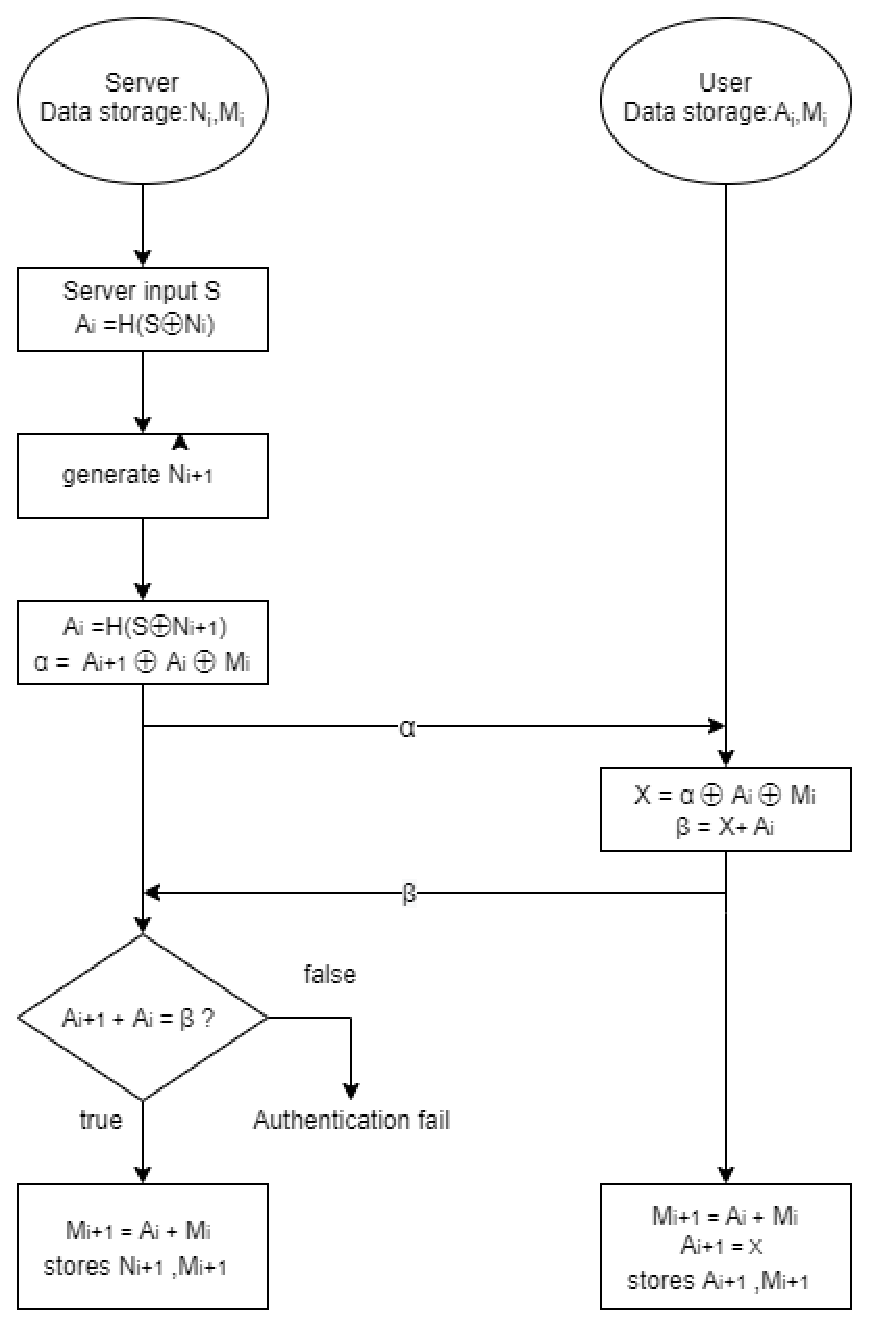
\includegraphics[scale=0.75]{./image/sasl4i.eps}
 \caption{SAS-L(4)の認証フェーズ}
 \label{4i}
\end{figure}
%



\section{SAS-L(3)}\label{SAS-L(3)}
SAS-L(3)は、SAS-L(4)と同様に、従来方式のSAS-2における被認証者側の演算負荷を改善する方式として清水明宏教授によって考案された。ただし、SAS-L(3)では、マスク値(秘匿情報)を用いない。SAS-L(3)はSAS-L(4)と同様に、初回認証の前に行われる登録フェーズと、認証フェーズに分かれていて、今回認証情報と次回認証情報の演算が同一になるかどうかを検証することで認証を行う。SAS-L(3)のアルゴリズムの詳細を次に示す。

\subsection{定義と表記法}
以下に、各フェーズを説明する際に使用する用語および記号の定義を記載する。
\begin{enumerate}[・]
%\item User とは、被認証者を表す。
				%\item Server とは、 User を認証する認証者を表す。
				\item 認証情報 とは、サーバとユーザで共有された認証に用いる情報表す。
				\item 今回認証情報 とは、現在のセッションで認証に用いる認証情報を表す。
				\item 次回認証情報 とは、次のセッションで認証に用いる新しい認証情報を表す。
				\item $i$ とは、セッションの回数を表す1以上の整数値を表す。
				\item S とは、 User の識別子を表す。
				\item H(s) とは、s に対して一方向性関数を1度適用し、得た演算結果を表す。
				%\item $N_1$とは、i初回の認証時に生成される乱数を表す。
				\item $N_i$とは、i 回目の認証時に生成される乱数を表す。
				\item $A_1$とは、初回認証情報を表す。
				\item $A_i$とは、i 回目のセッションで用いる今回認証情報を表す。
				%\item $M_i$とは、 i 回目の認証時に生成されるマスク値を表す。
				\item + とは、ビット毎の算術加算を表す。
				\item $\oplus$とは、 ビット毎の排他的論理和である。
\end{enumerate}
\subsection{初回登録フェーズ}
初回登録フェーズは以下の処理を安全な通信で行う。図\ref{3f}に初回登録フェーズのフローチャートを示す。

\textgt{サーバ}
\begin{enumerate}[1.]
\item ユーザ識別子 S を設定・保持する。
				\item 初回認証用の乱数 $N_1$ を生成し保存する。
				\item 入力されたS、 生成された $N_1$を用いて 初回認証用の認証情報$A_1 = H(S \oplus N_1)$ を演算し、保存する。
				\item 安全なルートを経由し、$A_1$をユーザへ送信する。
\end{enumerate}

\textgt{ユーザ}
\begin{enumerate}[1.]
\item 受け取った $A_1$ を保存する。
\end{enumerate}
%
\begin{figure}[H]
 \center
 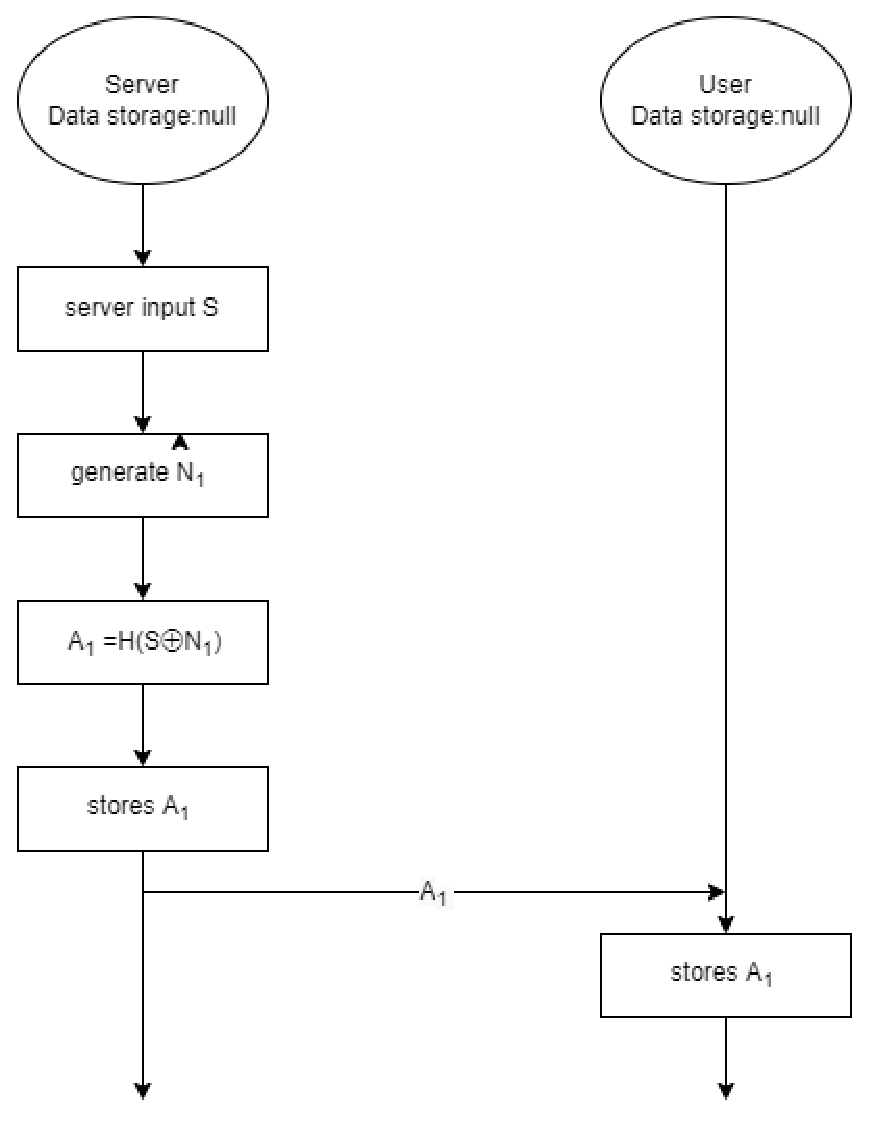
\includegraphics[scale=0.75]{./image/sasl3first.eps}
 \caption{SAS-L(3)の登録フェーズ}
 \label{3f}
\end{figure}
%




\subsection{認証フェーズ}
図\ref{3i}にi回目の認証フェーズのフローチャートを示す。

\textgt{サーバ}
\begin{enumerate}[1.]
				\item ユーザ識別子S 、乱数 $N_{i}$を入力する。
				\item 次回認証用の乱数 $N_{i+1}$を生成する。
				\item 乱数 $N_{i+1}$から次回認証用の認証情報 $A_{i+1} = H(S \oplus N_{i+1} )$、
				$\alpha = A_i \oplus A_{i+1} $を演算する。
				\item $\alpha$をユーザへ送信する。以降、認証情報送信に使用するネットワークはインターネット
				などの安全でないルートであっても問題はない。
				\item 受信した $\beta$  と 、 $A_i + A_{i+1}$ を比較し、 一致すれば認証が成功、 以下の処理が実行
				される。不一致ならば認証は不成立となり以下の処理は実行されない。
				%\item $M_{i+1}=A_i + M_i$を演算する。
				%$M_{i+1}$の演算を行う際に桁あふれを起こした場合はその値を切り捨てるものとする。
				\item 保存されている $A_i$ の代わりに $A_{i+1}$ を新しい認証情報として保存する。
				
\end{enumerate}

\textgt{ユーザ}
\begin{enumerate}[1.]
				\item 受信した$\alpha$と保存された $A_i$ を用いて $X = \alpha \oplus A_i ,\beta =X+A_i$を演算する。
				\item $\beta$ をサーバへ送信する。
				\item 保存されている $A_i$ の代わりに $A_{i+1}=X$ を新しい認証情報を保存する。
\end{enumerate}
%
\begin{figure}[H]
 \center
 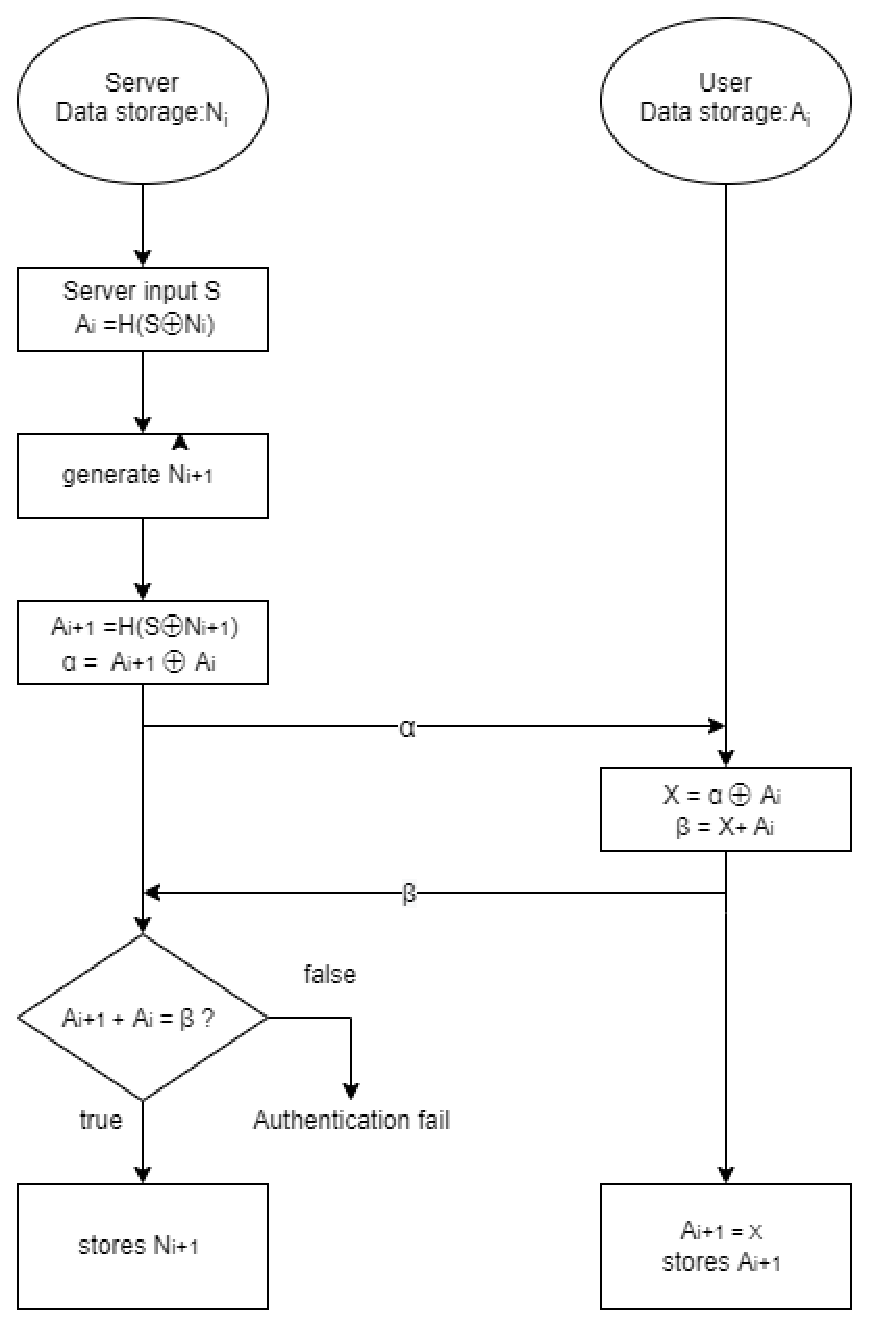
\includegraphics[scale=0.75]{./image/sasl3i2.eps}
 \caption{SAS-L(3)の認証フェーズ}
 \label{3i}
\end{figure}
%

\subsection{SAS-L認証方式の演算負荷比較}
SAS-(4)、SAS-L(3) に要求される計算回数を比較した表\ref{tb2}に示す。SAS-L(4)認証方式は、
ユーザ側において、一方向性変換の適用回数は 0 回、排他的論理和 (XOR) の適用回数が 2
回、加算の適用回数が2回である。
サーバ側においては一方向性変換の適用回数は 2 回、排他的論理和の適用回数は 4 回、加算の適用回数は2回である。
これに対して、SAS-L(3) はユーザ側において、一方向性変換の適用回数が 2 回、排他的論
理和の適用回数が 1回、加算の適用回数が 1 回である。
サーバ側においては一方向性変換の適用回数を 2 回、排他的論理和の適用回数は 3 回、加算の適用回数は 1 回である。
SAS-L(3)は、マスク値(秘匿情報)を用いないため、SAS-L(4)と比較して、排他的論理和の適用回数が2回、加算の適用回数が2回少ないことがわかる。よって理論上では、SAS-L(3)の方が演算負荷が軽量といえる。

		\begin{table}[H]
			\begin{center}
				\caption{演算負荷の比較表}
				\label{tb2} %表のラベルはcaptionの直下に置く
				\begin{tabular}{|l|c|c|c|c|c|c|}
					\hline
				   		& \multicolumn{3}{c|}{\textbf{被認証者側}}                                               & \multicolumn{3}{c|}{\textbf{認証者側}}                                               \\ \hline
				   		& \multicolumn{1}{l|}{一方向性関数} & \multicolumn{1}{l|}{XOR} & \multicolumn{1}{l|}{加算} & \multicolumn{1}{l|}{一方向性関数} & \multicolumn{1}{l|}{XOR} & \multicolumn{1}{l|}{加算} \\ \hline
					SAS-L(4) & 0                           & 2                        & 2                       & 2                           & 4                        & 2                       \\ \hline
					SAS-L(3) & 0                           & 1                        & 1                       & 2                           & 3                        & 1                       \\ \hline
				\end{tabular}
			\end{center}
		\end{table}


%-------------------------------------------------------------------------------------------
%-------------------------------------------------------------------------------------------
%-------------------------------------------------------------------------------------------



\section{安全性}
SAS-(3)の安全性の検証方法について述べる。認証フェーズにおいてユーザとサーバ間でのやり取りするデータ$\alpha$と$\beta$は、第3者は入手することができる。SAS-L(1)では、i回目、i+1回目、i+2回目のデータ$\alpha$と$\beta$を用いてi+3回目のデータを作成可能であり、過去のデータを再利用できるリプレイアタックの脅威がある。リプレイアタックとは、ネットワークを盗聴し認証情報を取得し、それらを別の機会にシステムに接続させるために用いる攻撃である\cite{SAS-L IoTに適した認証方式について}。
SAS-L(2)、SAS-L(4)では、マスク値(秘匿情報)を付加することで、リプレイアタックの脅威を回避している\cite{SAS}。 SAS-L(3)においては、安全性は未検証であるため、リプレイアタックの脅威を調べることで安全性の検証を行う。

まずSAS-L(3)のリプレイアタックの脅威において、SAS-L(1)同様に過去3回分の$\alpha$と$\beta$を利用されたときを検討する。例えば本実験例で、第i回目から第i+2回目の認証手順において、以下のデータが$\alpha$と$\beta$として送信される。
%を式\ref{eqn:11},式\ref{eqn:12}、i+1回目を式\ref{eqn:21},式\ref{eqn:22}、i+2回目を式\ref{eqn:31},式\ref{eqn:32}に示す。

\textgt{i回目}
\begin{equation}\label{eqn:11}
\alpha_i = A_{i} \oplus A_{i+1} 
\end{equation}
\begin{equation}\label{eqn:12}
\beta_i = A_{i} + A_{i+1} 
\end{equation}
%
\textgt{i+1回目}
\begin{equation}\label{eqn:21}
\alpha_{i+1} = A_{i+1} \oplus A_{i+2} 
\end{equation}
\begin{equation}\label{eqn:22}
\beta_{i+1} = A_{i+1} + A_{i+2} 
\end{equation}
%
\textgt{i+2回目}
\begin{equation}\label{eqn:31}
\alpha_{i+2} = A_{i+2} \oplus A_{i+3} 
\end{equation}
\begin{equation}\label{eqn:32}
\beta_{i+2} = A_{i+2} + A_{i+3} 
\end{equation}

%データ(\ref{eqn:11})から(\ref{eqn:32})に対して、
$\alpha_{i} \oplus \alpha_{i+1} \oplus \alpha_{i+2}$により
\begin{equation}\label{eqn:41}
A_{i} \oplus A_{i+3} 
\end{equation}
が生成できる。
また、$\beta_{i} - \beta_{i+1} + \beta_{i+2}$により
\begin{equation}\label{eqn:42}
A_{i} + A_{i+3} 
\end{equation}
が得られる。
SAS-L(1)の場合、式(\ref{eqn:41})、(\ref{eqn:42})を次のi+3回目の$\alpha_{i+3}$と$\beta_{i+3}$として入力すれば、認証が成立する\cite{SAS}。

SAS-L(3)についてi+3回目の認証を行うことを考える。サーバー側で作成した $\alpha_{i+3}$ が攻撃者により(\ref{eqn:41})式に置き換えられたとする。このとき攻撃者は次回認証情報を$A_i$にしようとしている。ユーザー側は(\ref{eqn:41})式を受け取り、ユーザー側で(\ref{eqn:42})式が計算される。ユーザーから(\ref{eqn:42})式がサーバ側に返されるが、サーバー側では正しい次回認証情報$A_{i+3}$を保存しており正しい$\beta_{i+3}$ つまり $A_{i+4}+A_{i+3}$ が計算できる。この計算結果は不正な(\ref{eqn:42})式とは異なるため認証が失敗する。つまり、SAS-L(3)ではSAS-L(1)で有効だったリプレイアタックは失敗する。

%しかしSAS-L(3)の場合、データ(\ref{eqn:41})、(\ref{eqn:42})を次のi+3回目の$\alpha$と$\beta$として入力しても、認証条件である$A_{i+3} + A_{i+4} $と一致しないため、認証不成立となる。SAS-L(3)では、i回目の認証に対して、認証条件に必ず$A_{i+1}$が必要なため、過去のデータの再利用が不可能でり、リプレイアタックの脅威がないといえる。
%また、SAS-L(3)において、$A_{i+1}  \oplus A_i$の各桁が1の場合、$A_{i+1}$と$A_{i}$は0,1か1,0のいずれかになる。0の場合、$A_{i+1}$と$A_{i}$は0,0か1,1のいずれかになる。したがって、$A_{i+1}$,$A_{i}$が64bitの場合、総当たりで$\beta$を確認すれば、最大$2^{64}$回のトライアルで$A_{i+1}$および$A_{i}$を特定できる。近年のコンピュータ技術の進展により、暗号方式が総当たりの暗号破りの危険性を回避するために、本実験では256bitの鍵長を用いることで総当たりの危険性を回避している。

%\section{同期問題対策手法}
%-------------------------------------------------------------------------------------------
%-------------------------------------------------------------------------------------------
%-------------------------------------------------------------------------------------------
\chapter{実験方法および評価実験}

\section{実装方法}

SAS-L(4),SAS-L(3)のプロトコルをC言語で実装する。また、ユーザとサーバ間の通信はソケット通信(Linuxの標準ライブラリのsocket関数)で実装した。

一方向性関数は、代表的なアルゴリズムとしてMD5、SHA256、SHA512などが存在する。MD5は同じハッシュ値を持つ入力値のペアが、一般的なPCで探索できてしまい、安全性が低いとされる。SHA256は、現在の安全性の基準である128ビット安全性を満足するため、本実装では一方向性関数としてOpenSSL内のSAH256を用いる。
乱数生成では、C言語で実装可能なOpenSSL内のRAND\_bytes()関数を用いる。

本研究では、CPU時間を計測しSAS-L(3)の計算時間の評価を行う。CPU時間の計測方法としてLinuxの標準ライブラリのclock関数を用いる。clock関数はCPUでかかった時間を計測するため、処理内容について複数回実行し評価する。


実行方法を付録Aに、ソースコードを付録Bに示す。
\section{計算機環境}
計算機環境について以下の表\ref{tab3}に示す。
\begin{table}[H]
		\begin{center}
			\caption{計算機環境}
			\label{tab3}
			\begin{tabular}{|l||l|}
				\hline
				\textbf{CPU}   & Intel(R) Core(TM) i5-7300U CPU @ 2.60GHz\\ \hline
				\textbf{メモリ}   & 8GB                    \\ \hline
				\textbf{ディスク} & 20GB                   \\ \hline
				\textbf{OS} &Linux7.9.2009             \\ \hline
			\end{tabular}
		\end{center}
\end{table}

	
\section{実験結果}
SAS-L(3),SAS-L(4)において、認証フェーズを1000回繰り返す実験を10回行い、計測したCPU計算時間の平均時間を表\ref{tb4}、表\ref{tb5}に示す。演算1では、加算、排他的論理和、一方向性関数、演算2では、加算、排他的論理和が含まれる。また、表\ref{tb4}、表\ref{tb5}を棒グラフにしたものを図\ref{4f}、図\ref{5f}に示す。


	\begin{table}[H]
		\begin{center}
			\caption{サーバ側の各認証方式における認証部1000回分のCPU時間(秒)}
			\label{tb4}
			\begin{tabular}{|c|c|c|c|c|c|}
				\hline
				%\multicolumn{1}{|l|}
				サーバ &全体& 乱数生成 & 通信 & 演算1\\ \hline \hline
				SAS-L(4)         & 0.0259        & 0.0048       & 0.0141&0.0070\\ \hline
				SAS-L(3)        & 0.0255       & 0.0048       & 0.0140&0.0067\\ \hline
			\end{tabular}
		\end{center}
	\end{table}
	
	
	\begin{table}[H]
		\begin{center}
			\caption{ユーザ側の各認証方式における認証部1000回分のCPU時間}
			\label{tb5}
			\begin{tabular}{|c|c|c|c|c|}
				\hline
				%\multicolumn{1}{|l|}
				ユーザ &全体& 通信 & 演算2\\ \hline \hline
				SAS-L(4)         & 0.0195      & 0.0160&0.0035\\ \hline
				SAS-L(3)        & 0.0191       & 0.0159&0.0032\\ \hline
			\end{tabular}
		\end{center}
	\end{table}
%
\begin{figure}[H]
 \center
 \includegraphics[scale=0.8]{./image/result.eps}
 \caption{認証フェーズ1000回のCPU計算時間(サーバ側)}
 \label{4f}
\end{figure}
%
%
\begin{figure}[H]
 \center
 \includegraphics[scale=0.8]{./image/result2.eps}
 \caption{認証フェーズ1000回のCPU計算時間(ユーザ側)}
 \label{5f}
\end{figure}
%

%サーバーの認証フェーズについては、表\ref{tb4}により、演算については計算時間に違いが見られ、SAS-L(3)が計算時間が短くなるという結果が得られた。しかしSAS-L(4)に比べXORが1回、加算が1回少ないだけなので、全体としての計算時間にほとんど差は見られない。
 %ユーザーの認証フェーズについては、表\ref{tb5}により、演算に含まれるXORと加算の回数は1/2になるはずであるが、SAS-L(3)はSAS-L(4)より0.0002秒だけ速く計算ができただけだった。この原因はclock関数の精度と関係するものと考えられる。より高い精度で計測できる関数を利用すると違いが明確になると考えられる。
 %以上のように、サーバー側でもユーザ側でもSAS-L3のほうが早く認証が行えることが確認できた。この理由はSAS-L3のほうがXORや加算の計算回数が少ないためである。実装コスト、計算時間と安全性の面でSAS-L3の有効性を確認することができた。

サーバーおよびユーザーの認証フェーズについて、SAS-L(3)がSAS-L(4)に比べて排他的論理和が1回、加算が1回少ない。そのため、表\ref{tb4}および表\ref{tb5}に示すように、SAS-L(3)のほうが短い計算時間で認証が行えることが確認できた。従って、演算回数、計算時間、安全性の面でSAS-L(3)の有効性を確認することができた。
 但し、ユーザーの認証フェーズの演算2(排他的論理和と加算)については、表3.1に示すように、SAS-L(3)の計算コストはSAS-L(4)の計算コストの1/2であるはずである。しかし計算時間を計測すると、SAS-L(3)の演算2の計算時間はSAS-L(4)の演算2の計算時間より0.0003秒だけ早く計算できるという結果になった。この点についてはより精度の高い時間の評価方法を用いて検討する必要がある。
	
		
%-------------------------------------------------------------------------------------------
%-------------------------------------------------------------------------------------------
%-------------------------------------------------------------------------------------------
\chapter{結論}
本研究では、ワンタイムパスワード認証方式SAS-L(3)の安全性を評価し、SAS-L(1)では存在したリプレイアタックの脅威がSAS-L(3)に存在しないことを確認した。さらに、SAS-L(3)を計算機上に実装し、SAS-L(4)と比較してサーバおよびユーザの認証フェーズの計算時間が短縮できることを示した。
 本研究ではSAS-L(3)をLinuxを搭載したPC上のみで検証したが、今後の課題として、
\begin{enumerate}[・]
				\item SAS-L(3)のIoT機器への実装や計算時間の評価
\end{enumerate}
があげられる。


%本研究では、ワンタイムパスワード認証方式のSAS-L(3)のリプレイアタックの脅威とCPU計算時間の検証を計算機上で実装し、評価した。SAS-L(3)では、マスク値(秘匿情報)を用いなくとも、リプレイアタックの脅威がないことを確認し、SAS-L(4)と比較してCPU計算時間の高速化を実現できた。

%また、本研究では計算機上のみでの検証であるため、実際にIoT機器に実装して検証することが今後の課題である。

%理論的には、SAS-L(3)のほうが演算の適用回数が少ないが、全体の処理時間を比較すると、1~2\%の高速化しか期待できず、これは演算以外の処理負荷が大きすぎることが原因であると決定づけた。

%また、本研究ではユーザとサーバ間の通信をソケット通信で行ったが、今回実装したソケット通信では1018回で停止していしまう問題がある。また、今回の通信の実装では比較的、処理負荷が大きかったため、別の通信方法を検討することも今後の課題である。
\acknowledgement

本研究を遂行するにあたり、常日頃より丁寧なご指導を頂きました、高橋寛教授、甲斐博准教授、王森レイ講師に深く御礼申し上げます。そして、本研究に際し、ご審査頂きました遠藤慶一准教授、宇戸寿幸准教授に深く御礼申し上げます。最後に、ご支援いただいた本学情報工学科の諸先生方、研究室の皆様に厚く御礼申し上げます。

\begin{thebibliography}{99}
%\bibitem{令和3年版情報通信白書}
%総務省,
%``デジタル計経済の進展とICT市場の動向,''\\
%令和3年度版情報通信白書,pp.43,2021.
%
\bibitem{サイバー攻撃の最近の動向等について}
サイバーセキュリティタスクフォース事務局,
``サイバー攻撃の最近の動向等について,令和2年12月3日''\\
\url{https://www.soumu.go.jp/main_content/000722477.pdf}(参照:2022-1-15)

%
%\bibitem{テスト}
%Kumar Sekhar Roy,Hemanta Kumar Kalita,\\
%``A Survey on Authentication Schemes in IoT,''\\
%Conference: 2017 International Conference on Information Technology (ICIT),Decemer 2017
%
\bibitem{SAS-Lワンタイムパスワード認証方式について}
清水明宏,
``SAS-Lワンタイムパスワード認証方式について,''
高知工科大学,\\
 preprint, 2020.
 %
\bibitem{認証技術}
Richard E. Smith,
``認証技術 パスワードから公開鍵まで,''
オーム社,2003.
 %
\bibitem{s/key}
Bellcore,
``The S/KEY One-Time Password System,''
RFC1760 Feb 1995.
 %
\bibitem{Lamport}
Leslie Lamport,
``Password authentication with insecure communication,''
Communications of the ACM, Volume 24,Issue 11,Nov.1981,pp770-772.
 %
 \bibitem{ハッシュ関数}
IPUSIRON,
``暗号技術のすべて,''
翔泳社,2017.
%
\bibitem{SAS}
清水明宏,
``SASワンタイムパスワード認証方式について,''
高知工科大学,\\
 スライド, 2021,10.
%
\end{thebibliography}

\appendix

\chapter{その他}
\section{実行方法}
認証情報が256bitの場合のコンパイル方法と実行方法は次の通りである。
	\begin{description}
		\item[認証者側]\mbox{} \\
    \;\;\;コンパイル方法は次の通りである。ここでは、ソースファイル名をsasl-4\_server.c、
			実行ファイル名をserverとする。openSSLのsha.hをインクルードするため、リンクオプションとして
			\verb|-lcrypto|を追加する。
			\begin{screen}
				\verb|% gcc sasl2server.c -o server -lcrypto|
			\end{screen}
			\;\;\;次に、実行方法は次の通りである。
				\begin{screen}
					\verb|% ./server|
				\end{screen}
			\item[被認証者側]\mbox{} \\
      \;\;\;コンパイル方法は次の通りである。ここでは、ソースファイル名をsas-4\_client.c、
				実行ファイル名をclientとする。次に示す例ではリンクオプション
				\verb|-lcrypto|が追加されているが、SAS-L(4)の被認証者側プログラムでは追加する必要はない。
				\begin{screen}
					\verb|% gcc sas2client.c -o client -lcrypto|
				\end{screen}
				\;\;\;次に、実行方法は次の通りである。
				\begin{screen}
					\verb|% ./client|
				\end{screen}	
	\end{description}
	SAS-L(3)においても、ソースファイル名が異なるだけで、同様の方法である。

\chapter{プログラムリスト}
%\begin{lstlisting}[caption = sasl-(4)\_server.c]
\section{SAS-L(4)}
\subsection{サーバ側の動作}
\fontsize{6.5pt}{5pt}
\begin{verbatim}

#include <sys/socket.h>
#include <netinet/in.h>
#include <arpa/inet.h>
#include <stdio.h>
#include <stdlib.h>
#include <string.h>
#include <unistd.h>
#include <openssl/sha.h>
#include <openssl/rand.h>
#include <time.h>

#define SERVER_ADDR "127.0.0.1"
#define SERVER_PORT 8080
#define BUF_SIZE 32

void xor(unsigned char result[],unsigned char x[],unsigned char y[],int len);
void add(unsigned char result[],unsigned char x[],unsigned char y[],int len);
void show(unsigned char s[],int len);
int transfer_first(int sock,unsigned char S[],unsigned char N1[],unsigned char M1[]);
int transfer_n(int sock,unsigned char S[],unsigned char N1[],unsigned char Mn[],clock_t *rand_clock,clock_t *sock_clock);

int main(void) {
  int w_addr, c_sock;
  struct sockaddr_in a_addr;
  unsigned char S[BUF_SIZE] = {0};//password
  unsigned char N1[BUF_SIZE] = {0};//rondom
  unsigned char M1[BUF_SIZE] = {0};//
  unsigned char Nn[BUF_SIZE] = {0};//rondom
  unsigned char Mn[BUF_SIZE] = {0};

  FILE *file;
  int i,cnt = 0;
  clock_t s_clock,e_clock,sum_clock = 0,rand_clock = 0,sock_clock = 0;

  /* ソケットを作成 */
  w_addr = socket(AF_INET, SOCK_STREAM, 0);
  if (w_addr == -1) {
    printf("socket error\n");
    return -1;
  }
  
  /* 構造体を全て0にセット */
  memset(&a_addr, 0, sizeof(struct sockaddr_in));

  /* サーバーのIPアドレスとポートの情報を設定 */
  a_addr.sin_family = AF_INET;
  a_addr.sin_port = htons((unsigned short)SERVER_PORT);
  a_addr.sin_addr.s_addr = inet_addr(SERVER_ADDR);

  /* ソケットに情報を設定 */
  if (bind(w_addr, (const struct sockaddr *)&a_addr, sizeof(a_addr)) == -1) {
    printf("bind error\n");
    close(w_addr);
    return -1;
  }

  /* ソケットを接続待ちに設定 */
  if (listen(w_addr, 3) == -1) {
    printf("listen error\n");
    close(w_addr);
    return -1;
  }
      
  //接続要求の受け付け(接続要求くるまで待ち)
  printf("Waiting connect...\n");
  c_sock = accept(w_addr, NULL, NULL);
  if (c_sock == -1) {
    printf("accept error\n");
    close(w_addr);
    return -1;
  }
  printf("Connected!!\n");

  printf("---初回登録---\n");
  //接続済のソケットでデータのやり取り
  transfer_first(c_sock,S,N1,M1);

    
  for(i = 0;i < BUF_SIZE;i++){
    Nn[i] = N1[i];
    Mn[i] = M1[i];
  }
    
  //------------------------------------------------
  while(cnt !=1000){
    //接続要求の受け付け(接続要求くるまで待ち)
    printf("Waiting connect...\n");
    c_sock = accept(w_addr, NULL, NULL);
    if (c_sock == -1) {
      printf("accept error\n");
      close(w_addr);
      return -1;
    }
    printf("Connected!!\n");
	    	    
    printf("---N回目認証---\n");

    printf("cnt:%d\n",cnt);
    
    s_clock  = clock();
    //接続済のソケットでデータのやり取り
    transfer_n(c_sock,S,Nn,Mn,&rand_clock,&sock_clock);

    e_clock  = clock();
    sum_clock = sum_clock + (e_clock - s_clock);

    cnt++;
  }
	      
  //ソケット通信をクローズ
  close(c_sock);

  printf("cnt:%d, sum_clock  :%f\n",cnt,(double)(sum_clock)/CLOCKS_PER_SEC);
  printf("cnt:%d, rand_clock :%f\n",cnt,(double)(rand_clock)/CLOCKS_PER_SEC);
  printf("cnt:%d, sock_clock :%f\n",cnt,(double)(sock_clock)/CLOCKS_PER_SEC);
  printf("cnt:%d, sum-ran-soc:%f\n",cnt,(double)(sum_clock - rand_clock - sock_clock)/CLOCKS_PER_SEC);

  /* 接続待ちソケットをクローズ */
  close(w_addr);

  return 0;
}

void xor(unsigned char result[],unsigned char x[],unsigned char y[],int len){
  int i;
  for(i=0;i< len;i++){
    result[i] = x[i] ^ y[i];
  }  
}

void add(unsigned char result[],unsigned char x[],unsigned char y[],int len){
  int i;
  for(i=0;i< len;i++){
    result[i] = x[i] + y[i];
  }  
}

void show(unsigned char s[],int len){
  int i;
  for(i=0;i< len;i++){
    printf("%02X",s[i]);
  }
  printf("\n");
}

int transfer_first(int sock,unsigned char S[],unsigned char N1[],unsigned char M1[]) {
  unsigned char send_buf[BUF_SIZE*2]={0};
  char recv_buf          ;
  int send_size, recv_size;  
  int i;

  SHA256_CTX sha_ctx;//コンテキストを生成

  unsigned char xor_result[BUF_SIZE] = {0};//result_xor
  unsigned char A1[BUF_SIZE] ={0};//hash
  FILE *fp;

  
  //  printf("パスワードを入力してください please password\n");
  //scanf("%s",S);

  
  //password  data -> S
  RAND_bytes(S,BUF_SIZE);
  //ランダムデータ random data -> N1
  RAND_bytes(N1,BUF_SIZE);
  //make M1
  RAND_bytes(M1,BUF_SIZE);

  //xor
  xor(xor_result,S,N1,sizeof(xor_result));

  //hash
  SHA256_Init(&sha_ctx);
  SHA256_Update(&sha_ctx,xor_result,sizeof(xor_result));
  SHA256_Final(A1,&sha_ctx);

  //print
  //printf("S     = ");
  //show(S,sizeof(S));
  //printf("N1    = ");
  //show(N1,sizeof(N1));
  //printf("A1    = ");
  //show(A1,sizeof(A1));
  //printf("M1    = ");
  //show(M1,sizeof(M1));

  //---------connect A1 M1----------
  for(i=0;i< BUF_SIZE;i++){
    send_buf[i] = A1[i];
  }
  int k = 0;
  for(i=BUF_SIZE;i< BUF_SIZE*2;i++){
    send_buf[i] = M1[k];
    k++;
  }
  //---------------------------------------
 
  /* 文字列を送信 */
  send_size = send(sock, send_buf, sizeof(send_buf) + 1, 0);
  if (send_size == -1) {
    printf("send error\n");
    return 0;
  }
  /* サーバーからの応答を受信 */
  recv_size = recv(sock, &recv_buf, 1, 0);
  if (recv_size == -1) {
    printf("recv error\n");
    return 0;
  }
  if (recv_size == 0) {
    /* 受信サイズが0の場合は相手が接続閉じていると判断 */
    printf("connection ended\n");
    return 0;
  }
  /* 応答が0の場合はデータ送信終了 */
  if (recv_buf == 0) {
    printf("接続を終了しました\n");
    return 0;
  }
  
  return 0;
}


int transfer_n(int sock,unsigned char S[],unsigned char Nn[],unsigned char Mn[],clock_t *rand_clock,clock_t *sock_clock) {
  unsigned char send_buf[BUF_SIZE]={0};
  unsigned char recv_buf[BUF_SIZE]={0};
  int send_size, recv_size;  
  int i;

  SHA256_CTX sha_ctx;//コンテキストを生成
  unsigned char Nn_next[BUF_SIZE] = {0};//N n+1
  unsigned char xor_result[BUF_SIZE] = {0};//result_xor
  unsigned char An[BUF_SIZE] ={0};
  unsigned char An_next[BUF_SIZE] ={0};
  unsigned char alpha[BUF_SIZE] ={0};
  unsigned char beta[BUF_SIZE] ={0};
  unsigned char Mn_next[BUF_SIZE] = {0};
  clock_t s_time,e_time;
  FILE *fp,*fp2;

  //printf("パスワードを入力してください please password\n");
  //scanf("%s",S);

  //printf("S=");
  //show(S,BUF_SIZE);
  //printf("Nn=");
  //show(Nn,BUF_SIZE);
  //printf("Mn=");
  //show(Mn,BUF_SIZE);
  
  
  /*----------make An----------*/
  //xor
  xor(xor_result,S,Nn,sizeof(xor_result));

  //hash
  SHA256_Init(&sha_ctx);
  SHA256_Update(&sha_ctx,xor_result,sizeof(xor_result));
  SHA256_Final(An,&sha_ctx);
 
  //----------generate Nn next----------
  s_time = clock();
  
  RAND_bytes(Nn_next,sizeof(Nn_next));

  e_time = clock();
  *rand_clock += (e_time - s_time);
  
  //----------make An_next----------
  //xor
  xor(xor_result,S,Nn_next,sizeof(xor_result));

  //hash
  SHA256_Init(&sha_ctx);
  SHA256_Update(&sha_ctx,xor_result,sizeof(xor_result));
  SHA256_Final(An_next,&sha_ctx);
  
  //----------make alpha----------
  xor(alpha,An_next,An,BUF_SIZE);
  xor(alpha,alpha,Mn,BUF_SIZE);
  
  //----------send_buf <- alpha----------
  for(i=0;i< BUF_SIZE;i++){
    send_buf[i] = alpha[i];
  }
  
  /*
  printf("An      = ");
  show(An,BUF_SIZE);
  printf("Mn      = ");
  show(Mn,BUF_SIZE);
  printf("Nn_next = ");
  show(Nn_next,sizeof(Nn_next));  
  printf("An_next = ");
  show(An_next,BUF_SIZE);
  printf("alpha   = ");
  show(alpha,BUF_SIZE);
  printf("send    = ");
  show(send_buf,BUF_SIZE+1);
  //----------make beta----------
  */
  add(beta,An_next,An,BUF_SIZE);
  /*
  printf("An+1 +An= ");
  show(beta,BUF_SIZE);
  */

  //----------send alpha  ----------
  s_time = clock();
  
  send_size = send(sock, send_buf , sizeof(send_buf) + 1, 0);
  if (send_size == -1) {
    printf("send error\n");
    return 0;
  }
  // clientからの応答を受信
  recv_size = recv(sock, recv_buf, BUF_SIZE, 0);
  if (recv_size == -1) {
    printf("recv error\n");
    return 0;
  }
  
  if (recv_size == 0) {
    //受信サイズが0の場合は相手が接続閉じていると判断 
    printf("connection ended\n");
    return 0;
  }
  //応答が0の場合はデータ送信終了
  if (recv_buf == 0) {
    printf("接続を終了しました\n");
    return 0;
  }

  e_time = clock();
  *sock_clock += (e_time - s_time);
  
  //------------------------------------------------

  int flag = 0;
  //xor
  for(i=0;i< BUF_SIZE;i++){
    if((recv_buf[i] ^ beta[i])!=0){
      flag= 1;
      break;
    }
    else{
      flag = 0;
    }
  }
  
  if(flag == 0){
    printf("認証成功\n");
    
    //----------make Mn_next----------
    //add
    add(Mn_next,An,Mn,sizeof(Mn_next));
    
    for(i = 0;i < BUF_SIZE;i++){
      Nn[i] = Nn_next[i];
      Mn[i] = Mn_next[i];
    }
    
  }
  else{
    printf("認証失敗\n");
  }

  return 0;
}

%\end{lstlisting}
\end{verbatim}


\subsection{ユーザ側の動作}
\fontsize{6.5pt}{5pt}
\begin{verbatim}

#include <sys/socket.h>
#include <netinet/in.h>
#include <arpa/inet.h>
#include <stdio.h>
#include <string.h>
#include <unistd.h>
#include <openssl/sha.h>
#include <openssl/rand.h>
#include <time.h>

#define SERVER_ADDR "127.0.0.1"
#define SERVER_PORT 8080
#define BUF_SIZE 32

void xor(unsigned char result[],unsigned char x[],unsigned char y[],int len);
void add(unsigned char result[],unsigned char x[],unsigned char y[],int len);
void show(unsigned char s[],int len);
int transfer_first(int sock,unsigned char A1[],unsigned char M1[]);
int transfer_n(int sock,unsigned char An[],unsigned char Mn[],clock_t *sock_clock);


int main(void) {
  int sock;
  struct sockaddr_in addr;
  FILE *file;
  int i,cnt=0;
  unsigned char A1[BUF_SIZE] = {0};
  unsigned char M1[BUF_SIZE] = {0};
  unsigned char An[BUF_SIZE] = {0};
  unsigned char Mn[BUF_SIZE] = {0};
  clock_t s_clock,e_clock,sum_clock = 0,sock_clock = 0;
  
  //---------------------------------------------
  /* ソケットを作成*/
  sock = socket(AF_INET, SOCK_STREAM, 0);
  if (sock == -1) {
    printf("socket error\n");
    return -1;
  }
  
  /* 構造体を全て0にセット */
  memset(&addr, 0, sizeof(struct sockaddr_in));
  
  /* サーバーのIPアドレスとポートの情報を設定*/
  addr.sin_family = AF_INET;
  addr.sin_port = htons((unsigned short)SERVER_PORT);
  addr.sin_addr.s_addr = inet_addr(SERVER_ADDR);
  
  /* サーバーに接続要求送信 */
  printf("接続を開始します...\n");
  if (connect(sock, (struct sockaddr*)&addr, sizeof(struct sockaddr_in)) == -1) {
    printf("connect error\n");
    close(sock);
    return -1;
  }
  printf("接続が完了しました!\n");
  //---------------------------------------------
  printf("---初回登録---\n");
  /* 初回登録時の接続済のソケットでデータのやり取り */

  transfer_first(sock,A1,M1);

  for(i = 0;i < BUF_SIZE;i++){
    An[i] = A1[i];
    Mn[i] = M1[i];
  }

  /* ソケット通信をクローズ */
  close(sock);
  
  printf("---N回目認証---\n");

  while(cnt !=1000){
    
    //ソケットを作成
    sock = socket(AF_INET, SOCK_STREAM, 0);
    if (sock == -1) {
      printf("socket error\n");
      return -1;
    }
    
    //構造体を全て0にセット 
    memset(&addr, 0, sizeof(struct sockaddr_in));
    
    //サーバーのIPアドレスとポートの情報を設定
    addr.sin_family = AF_INET;
    addr.sin_port = htons((unsigned short)SERVER_PORT);
    addr.sin_addr.s_addr = inet_addr(SERVER_ADDR);
    
    /* サーバーに接続要求送信 */
    printf("接続を開始します...\n");
    if (connect(sock, (struct sockaddr*)&addr, sizeof(struct sockaddr_in)) == -1) {
      printf("connect error\n");
      close(sock);
      return -1;
    }
    printf("接続が完了しました!\n");

    printf("cnt:%d\n",cnt);

    //---------------------------------------------
    s_clock = clock();
    
    /* N回目認証時の接続済のソケットでデータのやり取り */
    transfer_n(sock,An,Mn,&sock_clock);
    
    e_clock = clock();

    sum_clock = sum_clock + (e_clock - s_clock);

    
    /* ソケット通信をクローズ */
    close(sock);
    cnt++;
  }
   
  printf("cnt:%d, sum_clock :%f\n",cnt,(double)(sum_clock)/CLOCKS_PER_SEC);
  printf("cnt:%d, sock_clock:%f\n",cnt,(double)(sock_clock)/CLOCKS_PER_SEC);
  printf("cnt:%d, sock-sum  :%f\n",cnt,(double)(sum_clock - sock_clock)/CLOCKS_PER_SEC);
  return 0;
}


void xor(unsigned char result[],unsigned char x[],unsigned char y[],int len){
  int i;
  for(i=0;i< len;i++){
    result[i] = x[i] ^ y[i];
  }  
}

void add(unsigned char result[],unsigned char x[],unsigned char y[],int len){
  int i;
  for(i=0;i< len;i++){
    result[i] = x[i] + y[i];
  }  
}
 
void show(unsigned char s[],int len){
  int i;

  for(i=0;i< len;i++){
    printf("%02X",s[i]);
  }
  printf("\n");
}

int transfer_first(int sock,unsigned char A1[],unsigned char M1[]) {
  int recv_size, send_size,i;
  unsigned char recv_buf[BUF_SIZE*2];
  char send_buf;
 
  FILE *fp;
 
  /* クライアントから文字列を受信 */
  recv_size = recv(sock, recv_buf, BUF_SIZE*2, 0);
  if (recv_size == -1) {
    printf("recv error\n");
    return 0;
  }
  if (recv_size == 0) {
    /* 受信サイズが0の場合は相手が接続閉じていると判断 */
    printf("connection ended\n");
    return 0;
  }
    
  //A1
  for(i = 0;i < BUF_SIZE;i++){
    A1[i] = recv_buf[i];
  }
  
  //M1
  int k = 0;
  for(i = BUF_SIZE;i < BUF_SIZE*2;i++){
    M1[k] = recv_buf[i];
    k++;
  }

  //-------------------------------------------
  /* 接続終了を表す0を送信 */
  send_buf = 0;
  send_size = send(sock, &send_buf, 1, 0);
  if (send_size == -1) {
    printf("send error\n");
    return 0;
  }

  printf("接続を終了しました\n");
  return 0;
    
}

int transfer_n(int sock,unsigned char An[],unsigned char Mn[],clock_t *sock_clock) {
  int recv_size, send_size,i;
  unsigned char recv_buf[BUF_SIZE]={0};
  unsigned char send_buf[BUF_SIZE]={0};
  unsigned char An_next[BUF_SIZE] ={0};
  unsigned char Mn_next[BUF_SIZE] ={0};
  unsigned char alpha[BUF_SIZE] ={0};
  unsigned char beta[BUF_SIZE] ={0};
  clock_t s_time,e_time;
  FILE *fp;
  
  //----------receve alpha----------
  s_time = clock();
  
  // serverから文字列を受信
  recv_size = recv(sock, recv_buf, BUF_SIZE, 0);
  if (recv_size == -1) {
    printf("recv error\n");
    return 0;
  }
  if (recv_size == 0) {
    // 受信サイズが0の場合は相手が接続閉じていると判断
    printf("connection ended\n");
    return 0;
  }

  e_time = clock();
  *sock_clock += (e_time - s_time);
  
  //alpha
  for(i = 0;i < BUF_SIZE;i++){
    alpha[i] = recv_buf[i];
  }
  
  //----------make beta---------- 
  xor(beta,alpha,An,BUF_SIZE);
  xor(An_next,beta,Mn,BUF_SIZE);//make An_next
  add(beta,An_next,An,BUF_SIZE);

  /*
  //print
  printf("An      = ");
  show(An,BUF_SIZE);
  printf("An+1    = ");
  show(An_next,BUF_SIZE);
  printf("alpha   = ");
  show(alpha,BUF_SIZE);
  printf("beta?   = ");
  show(beta,BUF_SIZE);
  */


  //----------send beta---------
  s_time = clock();
  
  for(i = 0;i < BUF_SIZE;i++){
    send_buf[i] = beta[i];
  }
  send_size = send(sock, send_buf, BUF_SIZE, 0);
  if (send_size == -1) {
    printf("send error\n");
    return -1;
  }

  e_time = clock();
  *sock_clock += (e_time - s_time);
  
  //----------make Mn_next----------
  add(Mn_next,An,Mn,sizeof(Mn_next));

  for(i = 0;i < BUF_SIZE;i++){
    An[i] = An_next[i];
    Mn[i] = Mn_next[i];
  }

  printf("接続を終了しました\n");
  return 0;
 
}

\end{verbatim}

%\end{lstlisting}
%\begin{lstlisting}[caption = sas-(3)\_server.c]
\section{SAS-L(3)}
\subsection{サーバ側の動作}
\fontsize{6.5pt}{5pt}
\begin{verbatim}

#include <sys/socket.h>
#include <netinet/in.h>
#include <arpa/inet.h>
#include <stdio.h>
#include <stdlib.h>
#include <string.h>
#include <unistd.h>
#include <openssl/sha.h>
#include <openssl/rand.h>
#include <time.h>

#define SERVER_ADDR "127.0.0.1"
#define SERVER_PORT 8080
#define BUF_SIZE 32

void xor(unsigned char result[],unsigned char x[],unsigned char y[],int len);
void add(unsigned char result[],unsigned char x[],unsigned char y[],int len);
void show(unsigned char s[],int len);
int transfer_first(int sock,unsigned char S[],unsigned char N1[]);
int transfer_n(int sock,unsigned char S[],unsigned char N1[],clock_t *rand_clock,clock_t *sock_clock);

int main(void) {
  int w_addr, c_sock;
  struct sockaddr_in a_addr;
  unsigned char S[BUF_SIZE] = {0};//password
  unsigned char N1[BUF_SIZE] = {0};//rondom
  unsigned char Nn[BUF_SIZE] = {0};//rondom

  FILE *file;
  int i,cnt = 0;
  clock_t s_clock,e_clock,sum_clock = 0,rand_clock = 0,sock_clock = 0;

    /* ソケットを作成 */
    w_addr = socket(AF_INET, SOCK_STREAM, 0);
    if (w_addr == -1) {
        printf("socket error\n");
        return -1;
    }

    /* 構造体を全て0にセット */
    memset(&a_addr, 0, sizeof(struct sockaddr_in));

    /* サーバーのIPアドレスとポートの情報を設定 */
    a_addr.sin_family = AF_INET;
    a_addr.sin_port = htons((unsigned short)SERVER_PORT);
    a_addr.sin_addr.s_addr = inet_addr(SERVER_ADDR);

    /* ソケットに情報を設定 */
    if (bind(w_addr, (const struct sockaddr *)&a_addr, sizeof(a_addr)) == -1) {
        printf("bind error\n");
        close(w_addr);
        return -1;
    }

    /* ソケットを接続待ちに設定 */
    if (listen(w_addr, 3) == -1) {
        printf("listen error\n");
        close(w_addr);
        return -1;
    }
      
    //接続要求の受け付け(接続要求くるまで待ち)
    printf("Waiting connect...\n");
    c_sock = accept(w_addr, NULL, NULL);
    if (c_sock == -1) {
      printf("accept error\n");
      close(w_addr);
      return -1;
    }
    printf("Connected!!\n");

    printf("---初回登録---\n");
    //接続済のソケットでデータのやり取り
    transfer_first(c_sock,S,N1);

    
    for(i = 0;i < BUF_SIZE;i++){
      Nn[i] = N1[i];
    }
    
    //------------------------------------------------
    while(cnt !=1000){
      //接続要求の受け付け(接続要求くるまで待ち)
      printf("Waiting connect...\n");
      c_sock = accept(w_addr, NULL, NULL);
      if (c_sock == -1) {
	printf("accept error\n");
	close(w_addr);
	return -1;
      }
      printf("Connected!!\n");
	    	    
      printf("---N回目認証---\n");

      printf("cnt:%d\n",cnt);      
      s_clock  = clock();
          
      //接続済のソケットでデータのやり取り
      transfer_n(c_sock,S,Nn,&rand_clock,&sock_clock);

      e_clock  = clock();
      sum_clock += (e_clock - s_clock);

      cnt++;
    }
	      
    //ソケット通信をクローズ
    close(c_sock);
    
    printf("cnt:%d, sum_clock  :%f\n",cnt,(double)(sum_clock)/CLOCKS_PER_SEC);
    printf("cnt:%d, rand_clock :%f\n",cnt,(double)(rand_clock)/CLOCKS_PER_SEC);
    printf("cnt:%d, sock_clock :%f\n",cnt,(double)(sock_clock)/CLOCKS_PER_SEC);
    printf("cnt:%d, sum-ran-soc:%f\n",cnt,(double)(sum_clock - rand_clock - sock_clock)/CLOCKS_PER_SEC);
    /* 接続待ちソケットをクローズ */
    close(w_addr);

    return 0;
}

void xor(unsigned char result[],unsigned char x[],unsigned char y[],int len){
  int i;
  for(i=0;i< len;i++){
    result[i] = x[i] ^ y[i];
  }  
}

void add(unsigned char result[],unsigned char x[],unsigned char y[],int len){
  int i;
  for(i=0;i< len;i++){
    result[i] = x[i] + y[i];
  }  
}

void show(unsigned char s[],int len){
  int i;
  for(i=0;i< len;i++){
    printf("%02X",s[i]);
  }
  printf("\n");
}

int transfer_first(int sock,unsigned char S[],unsigned char N1[]) {
  unsigned char send_buf[BUF_SIZE]={0};
  char recv_buf          ;
  int send_size, recv_size;  
  int i;

  SHA256_CTX sha_ctx;//コンテキストを生成

  unsigned char xor_result[BUF_SIZE] = {0};//result_xor
  unsigned char A1[BUF_SIZE] ={0};//hash
  FILE *fp;

  
  //  printf("パスワードを入力してください please password\n");
  //scanf("%s",S);

  
  //password  data -> S
  RAND_bytes(S,BUF_SIZE);
  //ランダムデータ random data -> N1
  RAND_bytes(N1,BUF_SIZE);

  //xor
  xor(xor_result,S,N1,sizeof(xor_result));

  //hash
  SHA256_Init(&sha_ctx);
  SHA256_Update(&sha_ctx,xor_result,sizeof(xor_result));
  SHA256_Final(A1,&sha_ctx);

  //print
  //printf("S     = ");
  //show(S,sizeof(S));
  //printf("N1    = ");
  //show(N1,sizeof(N1));
  //printf("A1    = ");
  //show(A1,sizeof(A1));
  //printf("M1    = ");
  //show(M1,sizeof(M1));

  //---------connect A1 M1----------
  for(i=0;i< BUF_SIZE;i++){
    send_buf[i] = A1[i];
  }

  //---------------------------------------
 
  /* 文字列を送信 */
  send_size = send(sock, send_buf, sizeof(send_buf) + 1, 0);
  if (send_size == -1) {
    printf("send error\n");
    return 0;
  }
  /* サーバーからの応答を受信 */
  recv_size = recv(sock, &recv_buf, 1, 0);
  if (recv_size == -1) {
    printf("recv error\n");
    return 0;
  }
  if (recv_size == 0) {
    /* 受信サイズが0の場合は相手が接続閉じていると判断 */
    printf("connection ended\n");
    return 0;
  }
  /* 応答が0の場合はデータ送信終了 */
  if (recv_buf == 0) {
    printf("接続を終了しました\n");
    return 0;
  }
  
  return 0;
}


int transfer_n(int sock,unsigned char S[],unsigned char Nn[],clock_t *rand_clock,clock_t *sock_clock) {
  unsigned char send_buf[BUF_SIZE]={0};
  unsigned char recv_buf[BUF_SIZE]={0};
  int send_size, recv_size;  
  int i;

  SHA256_CTX sha_ctx;//コンテキストを生成
  unsigned char Nn_next[BUF_SIZE] = {0};//N n+1
  unsigned char xor_result[BUF_SIZE] = {0};//result_xor
  unsigned char An[BUF_SIZE] ={0};
  unsigned char An_next[BUF_SIZE] ={0};
  unsigned char alpha[BUF_SIZE] ={0};
  unsigned char beta[BUF_SIZE] ={0};
  clock_t s_time,e_time;
  FILE *fp,*fp2;

  //printf("パスワードを入力してください please password\n");
  //scanf("%s",S);

  //printf("S=");
  //show(S,BUF_SIZE);
  //printf("Nn=");
  //show(Nn,BUF_SIZE);
  //printf("Mn=");
  //show(Mn,BUF_SIZE);
  
  
  /*----------make An----------*/
  //xor
  xor(xor_result,S,Nn,sizeof(xor_result));

  //hash
  SHA256_Init(&sha_ctx);
  SHA256_Update(&sha_ctx,xor_result,sizeof(xor_result));
  SHA256_Final(An,&sha_ctx);
 
  //----------generate Nn next----------
  s_time = clock();

  RAND_bytes(Nn_next,sizeof(Nn_next));

  e_time = clock();
  *rand_clock += (e_time - s_time);
  //----------make An_next----------
  //xor
  xor(xor_result,S,Nn_next,sizeof(xor_result));

  //hash
  SHA256_Init(&sha_ctx);
  SHA256_Update(&sha_ctx,xor_result,sizeof(xor_result));
  SHA256_Final(An_next,&sha_ctx);
  
  //----------make alpha----------
  xor(alpha,An_next,An,BUF_SIZE);
  
  //----------send_buf <- alpha----------
  for(i=0;i< BUF_SIZE;i++){
    send_buf[i] = alpha[i];
  }
  
  
  //printf("An      = ");
  //show(An,BUF_SIZE);
  //printf("Mn      = ");
  //show(Mn,BUF_SIZE);
  //printf("Nn_next = ");
  //show(Nn_next,sizeof(Nn_next));  
  //printf("An_next = ");
  //show(An_next,BUF_SIZE);
  //printf("alpha   = ");
  //show(alpha,BUF_SIZE);
  
  //printf("send    = ");
  //show(send_buf,BUF_SIZE);
  //----------make beta----------
  
  add(beta,An_next,An,BUF_SIZE);
  
  //printf("An+1 +An= ");
  //show(beta,BUF_SIZE);
  

    //----------send alpha  ----------

  s_time = clock();
  send_size = send(sock, send_buf , sizeof(send_buf) + 1, 0);
  if (send_size == -1) {
    printf("send error\n");
    return 0;
  }
  // clientからの応答を受信
  recv_size = recv(sock, recv_buf, BUF_SIZE, 0);
  if (recv_size == -1) {
    printf("recv error\n");
    return 0;
  }
  
  if (recv_size == 0) {
    //受信サイズが0の場合は相手が接続閉じていると判断 
    printf("connection ended\n");
    return 0;
  }
  //応答が0の場合はデータ送信終了
  if (recv_buf == 0) {
    printf("接続を終了しました\n");
    return 0;
  }

  e_time = clock();
  *sock_clock += (e_time - s_time);
  //------------------------------------------------

  int flag = 0;
  //xor
  for(i=0;i< BUF_SIZE;i++){
    if((recv_buf[i] ^ beta[i])!=0){
      flag= 1;
      break;
    }
    else{
      flag = 0;
    }
  }
  
  if(flag == 0){
    printf("認証成功\n");
    
    for(i = 0;i < BUF_SIZE;i++){
      Nn[i] = Nn_next[i];
    }
    

  }
  else{
    printf("認証失敗\n");
  }

  return 0;
}
\end{verbatim}

\subsection{ユーザ側の動作}
\fontsize{6.5pt}{5pt}
\begin{verbatim}

%\end{lstlisting}
%\begin{lstlisting}[caption = sasl-(3)\_client.c]
#include <sys/socket.h>
#include <netinet/in.h>
#include <arpa/inet.h>
#include <stdio.h>
#include <string.h>
#include <unistd.h>
#include <openssl/sha.h>
#include <openssl/rand.h>
#include <time.h>

#define SERVER_ADDR "127.0.0.1"
#define SERVER_PORT 8080
#define BUF_SIZE 32

void xor(unsigned char result[],unsigned char x[],unsigned char y[],int len);
void add(unsigned char result[],unsigned char x[],unsigned char y[],int len);
void show(unsigned char s[],int len);
int transfer_first(int sock,unsigned char A1[]);
int transfer_n(int sock,unsigned char An[],clock_t *sock_clock);


int main(void) {
  int sock;
  struct sockaddr_in addr;
  FILE *file;
  int i,cnt=0;
  unsigned char A1[BUF_SIZE] = {0};
  unsigned char An[BUF_SIZE] = {0};
  clock_t s_clock,e_clock,sum_clock = 0,sock_clock = 0;
  
  //---------------------------------------------
  /* ソケットを作成*/
  sock = socket(AF_INET, SOCK_STREAM, 0);
  if (sock == -1) {
    printf("socket error\n");
    return -1;
  }
  
  /* 構造体を全て0にセット */
  memset(&addr, 0, sizeof(struct sockaddr_in));
  
  /* サーバーのIPアドレスとポートの情報を設定*/
  addr.sin_family = AF_INET;
  addr.sin_port = htons((unsigned short)SERVER_PORT);
  addr.sin_addr.s_addr = inet_addr(SERVER_ADDR);
  
  /* サーバーに接続要求送信 */
  printf("接続を開始します...\n");
  if (connect(sock, (struct sockaddr*)&addr, sizeof(struct sockaddr_in)) == -1) {
    printf("connect error\n");
    close(sock);
    return -1;
  }
  printf("接続が完了しました!\n");
  //---------------------------------------------
  printf("---初回登録---\n");
  /* 初回登録時の接続済のソケットでデータのやり取り */

  transfer_first(sock,A1);

  for(i = 0;i < BUF_SIZE;i++){
    An[i] = A1[i];
  }

  /* ソケット通信をクローズ */
  close(sock);
  
  printf("---N回目認証---\n");

  while(cnt !=1000){
    
    //ソケットを作成
    sock = socket(AF_INET, SOCK_STREAM, 0);
    if (sock == -1) {
      printf("socket error\n");
      return -1;
    }
    
    //構造体を全て0にセット 
    memset(&addr, 0, sizeof(struct sockaddr_in));
    
    //サーバーのIPアドレスとポートの情報を設定
    addr.sin_family = AF_INET;
    addr.sin_port = htons((unsigned short)SERVER_PORT);
    addr.sin_addr.s_addr = inet_addr(SERVER_ADDR);
    
    /* サーバーに接続要求送信 */
    printf("接続を開始します...\n");
    if (connect(sock, (struct sockaddr*)&addr, sizeof(struct sockaddr_in)) == -1) {
      printf("connect error\n");
      close(sock);
      return -1;
    }
    printf("接続が完了しました!\n");

    printf("cnt:%d\n",cnt);
    
    //---------------------------------------------
    s_clock = clock();
    
    /* N回目認証時の接続済のソケットでデータのやり取り */
    transfer_n(sock,An,&sock_clock);
    
    e_clock = clock();

    sum_clock += (e_clock - s_clock);

    /* ソケット通信をクローズ */
    close(sock);
    cnt++;
  }
  printf("cnt:%d, sum_clock :%f\n",cnt,(double)(sum_clock)/CLOCKS_PER_SEC);
  printf("cnt:%d, sock_clock:%f\n",cnt,(double)(sock_clock)/CLOCKS_PER_SEC);
  printf("cnt:%d, sock-sum  :%f\n",cnt,(double)(sum_clock - sock_clock)/CLOCKS_PER_SEC);
  return 0;
}


void xor(unsigned char result[],unsigned char x[],unsigned char y[],int len){
  int i;
  for(i=0;i< len;i++){
    result[i] = x[i] ^ y[i];
  }  
}

void add(unsigned char result[],unsigned char x[],unsigned char y[],int len){
  int i;
  for(i=0;i< len;i++){
    result[i] = x[i] + y[i];
  }  
}
 
void show(unsigned char s[],int len){
  int i;

  for(i=0;i< len;i++){
    printf("%02X",s[i]);
  }
  printf("\n");
}

int transfer_first(int sock,unsigned char A1[]) {
  int recv_size, send_size,i;
  unsigned char recv_buf[BUF_SIZE];
  char send_buf;
 
  FILE *fp;
 
  /* クライアントから文字列を受信 */
  recv_size = recv(sock, recv_buf, BUF_SIZE, 0);
  if (recv_size == -1) {
    printf("recv error\n");
    return 0;
  }
  if (recv_size == 0) {
    /* 受信サイズが0の場合は相手が接続閉じていると判断 */
    printf("connection ended\n");
    return 0;
  }
    
  //A1
  for(i = 0;i < BUF_SIZE;i++){
    A1[i] = recv_buf[i];
  }

  //-------------------------------------------
  /* 接続終了を表す0を送信 */
  send_buf = 0;
  send_size = send(sock, &send_buf, 1, 0);
  if (send_size == -1) {
    printf("send error\n");
    return 0;
  }

  printf("接続を終了しました\n");
  return 0;
    
}

int transfer_n(int sock,unsigned char An[],clock_t *sock_clock) {
  int recv_size, send_size,i;
  unsigned char recv_buf[BUF_SIZE]={0};
  unsigned char send_buf[BUF_SIZE]={0};
  unsigned char An_next[BUF_SIZE] ={0};
  unsigned char alpha[BUF_SIZE] ={0};
  unsigned char beta[BUF_SIZE] ={0};
  FILE *fp;
  clock_t s_time,e_time;
  //----------receve alpha---------- 
  // serverから文字列を受信
  s_time = clock();
  
  recv_size = recv(sock, recv_buf, BUF_SIZE, 0);
  if (recv_size == -1) {
    printf("recv error\n");
    return 0;
  }
  if (recv_size == 0) {
    // 受信サイズが0の場合は相手が接続閉じていると判断
    printf("connection ended\n");
    return 0;
  }

  e_time = clock();
  *sock_clock += (e_time - s_time);
  
  //alpha
  for(i = 0;i < BUF_SIZE;i++){
    alpha[i] = recv_buf[i];
  }

  //----------make beta---------- 
  xor(An_next,alpha,An,BUF_SIZE);
  add(beta,An_next,An,BUF_SIZE);

  
  //print
  /*
  printf("An      = ");
  show(An,BUF_SIZE);
  printf("An+1    = ");
  show(An_next,BUF_SIZE);
  printf("alpha   = ");
  show(alpha,BUF_SIZE);
  printf("beta?   = ");
  show(beta,BUF_SIZE);
  */


  //----------send beta---------
  s_time = clock();
  
  for(i = 0;i < BUF_SIZE;i++){
    send_buf[i] = beta[i];
  }
  send_size = send(sock, send_buf, BUF_SIZE, 0);
  if (send_size == -1) {
    printf("send error\n");
    return -1;
  }

  e_time = clock();
  *sock_clock += (e_time - s_time);
  
  for(i = 0;i < BUF_SIZE;i++){
    An[i] = An_next[i];
  }

  printf("接続を終了しました\n");
  return 0;
 
}
\end{verbatim}

%\end{lstlisting}



\end{document}


